\section{Results}
\label{sec:results}

\subsection{Overall Outcomes}

The outcomes of the five systems on the 150 test questions are given in
Table~\ref{tab:outcomes}, together with the precision when answering, that is, the
share of answered questions that were answered correctly. The full agent answered
\nFullCorrect\% of the questions correctly, was wrong on \nFullWrong\% and abstained on
\nFullAbstain\%. Single-pass, which never abstains, was correct on \nSPCorrect\% and
wrong on \nSPWrong\%.

\begin{table}[!htb]
\centering
\caption{Outcomes on the 150 test questions in percent, with 95\% bootstrap intervals
in brackets, and precision when answering (Prec.)}
\label{tab:outcomes}
\footnotesize
% generated by scripts/make_conference_tables.py -- do not edit
\setlength{\tabcolsep}{3.5pt}
\begin{tabular}{lcccc}
\toprule
System & Correct & Wrong & Abstained & Prec. \\
\midrule
Full (7B) & 21 [15, 28] & 43 [35, 51] & 35 [28, 43] & 33 \\
Single-pass & 34 [27, 41] & 66 [59, 73] & 0 [0, 0] & 34 \\
Text-only & 15 [10, 21] & 51 [43, 59] & 33 [26, 41] & 23 \\
Strict G1 & 5 [2, 9] & 9 [5, 14] & 85 [79, 91] & 36 \\
Full (Gemini) & 30 [23, 37] & 51 [43, 59] & 19 [13, 26] & 37 \\
\bottomrule
\end{tabular}

\end{table}

The same outcomes are drawn in Fig.~\ref{fig:outcomes}, where the trade made by each
system can be seen directly: the gated systems replace part of the wrong answers with
abstentions, and the strict design replaces most answers of every kind.

\begin{figure}[!htb]
\centering
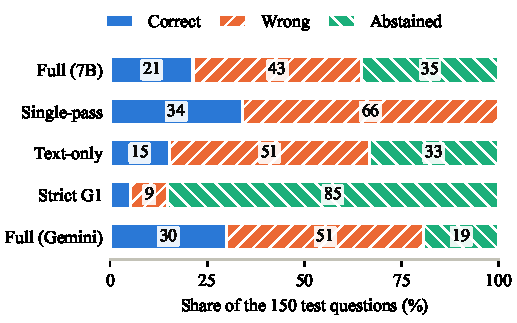
\includegraphics[width=\columnwidth]{figures/fig_outcomes.pdf}
\caption{Share of correct, wrong and abstained answers for each system on the 150 test
questions. Hatching distinguishes the outcomes in grey-scale print.}
\label{fig:outcomes}
\end{figure}

The judge was found to be reliable. It agreed with the human grader on \nJudgeAgree{}
answers (Cohen's kappa of \nJudgeKappa), and \nJudgeUnsure{}
further answers were left undecided by the grader. In all three disagreements, the
answer was accepted by the human and rejected by the judge, so the correct rates in
Table~\ref{tab:outcomes} are, if anything, conservative.

\subsection{RQ1: Agency}

The paired differences between the systems are listed in Table~\ref{tab:differences}.
Compared with single-pass, the full agent was wrong \nDiffWrongSP{} percentage points
less often, and the difference lies outside the bootstrap interval. It was also
correct \nDiffCorrectSP{} points less often, because \nFullAbstain\% of the questions
were left unanswered. Its precision when answering (\nFullPrec\%) was no higher than
that of single-pass (\nSPPrec\%), which shows that fewer wrong answers were obtained by
answering less rather than by answering better.

\begin{table}[!htb]
\centering
\caption{Paired differences in percentage points on the same questions
($^{*}$: the 95\% bootstrap interval excludes zero; MH: multi-hop subset)}
\label{tab:differences}
\footnotesize
% generated by scripts/make_conference_tables.py -- do not edit
\begin{tabular}{lccc}
\toprule
Comparison & Correct & Wrong & Abstained \\
\midrule
Full $-$ Single-pass & $-12.7$$^{*}$ & $-22.7$$^{*}$ & $+35.3$$^{*}$ \\
Full $-$ Text-only & $+6.0$ & $-8.0$ & $+2.0$ \\
Full $-$ Strict G1 & $+16.0$$^{*}$ & $+34.0$$^{*}$ & $-50.0$$^{*}$ \\
Gemini $-$ Full (7B) & $+8.7$ & $+7.3$ & $-16.0$$^{*}$ \\
\midrule
Full $-$ Single-pass, MH & $+20.0$ & $-40.0$$^{*}$ & $+20.0$ \\
Full $-$ Text-only, MH & $+40.0$$^{*}$ & $+0.0$ & $-40.0$$^{*}$ \\
\bottomrule
\end{tabular}

\end{table}

Whether the abstentions fall on the hard questions was tested with single-pass as a
reference. A selective agent would hold back the questions that single-pass also gets
wrong. The opposite was observed: single-pass was correct on \nSelFullHeld\% of the
questions that the full agent held back, but on only \nSelFullAns\% of those it answered.
The best-effort flag carried little information as well, since flagged answers were
correct about as often as those accepted by G1 (24 of 75 against 8 of 22). On the
multi-hop subset, where the loop was expected to matter most, the full agent was wrong
on 2 of the 10 questions against 6 for single-pass, but ten questions allow only an
indicative reading. The search tools were called 2.7 times per question by the agent and
3 times by single-pass, which gives a higher efficiency score (AES 0.44 against 0.36).
The planner and the gates, however, raised the number of model calls from 3 to 11.7
per question.

\subsection{A Change Made During Evaluation}
\label{sec:best-effort}

In its first frozen form, the agent abstained whenever G1 was not convinced after three
rounds. In the first test run, 110 of the first 142 questions were abstained before a
power cut stopped the run, although the reference was in the buffer for about two
thirds of them. The best-effort rule of Section~\ref{sec:method} was then designed on
the development split only, without any test answer being read; on that split it
moved the agent from 6 right, 1 partly right, 0 wrong and 13 abstained to 9, 4, 5 and
2. All systems were re-run on the test split, and the first design was kept as the
strict G1 ablation.

\subsection{RQ2: Visual Retrieval}

The reference table or figure reached the buffer for 73\% of the questions with the
full agent and for 77\% with single-pass, which fetches every kind of evidence in every
run. Of the distinct tables and figures fetched by the agent, 44\% were the reference
(RF 0.44, against 0.41 for single-pass and 0.55 with Gemini). On the development
split, ColQwen2 ranked the reference's page first for 15 of 20 questions. Compared with the text-only agent, the full agent was correct 6 points more
often and wrong 8 points less often (Table~\ref{tab:differences}), and neither
difference lies outside its interval. On the multi-hop subset, however, the full agent
was correct 40 points more often.

\subsection{RQ3: Grounding}
\label{sec:rq3}

The grounding scores on the 50 annotated questions are given in
Table~\ref{tab:grounding}. Measured by IoU, grounding was poor for every system. On
inspection, a correct proof was often scored low because it was drawn at a different
size: a parsed cell spans the width of its column, while the hand box was drawn
tightly around the printed number, so that two exactly right cells scored IoU 0.43 and
0.46. Shrinking each cited cell to its printed words did not raise CGS (0.070 against
0.068), as many questions lost as gained. The pointing game removes this effect, and it
credits the full agent on \nPointFullAns{} of its answered questions.

\begin{table}[!htb]
\centering
\caption{Grounding on the 50 annotated questions (CGS: best IoU; Point.: pointing game,
all and answered questions) and reference attribution on all 150 questions}
\label{tab:grounding}
\footnotesize
% generated by scripts/make_conference_tables.py -- do not edit
\begin{tabular}{lcccc}
\toprule
System & CGS & Point. & Point.\ (ans.) & Ref.\ attr. \\
\midrule
Full (7B) & 0.07 & 0.16 & 0.28 & 0.44 \\
Single-pass & 0.15 & 0.40 & 0.40 & 0.42 \\
Text-only & 0.00 & 0.04 & 0.07 & 0.00 \\
Full (Gemini) & 0.05 & 0.20 & 0.26 & 0.55 \\
\bottomrule
\end{tabular}

\end{table}

The low scores were traced to the choice of sources rather than to the boxes. Of the
\nProofBoxesFull{} proof boxes drawn by the full agent on the annotated questions, only
\nProofOnRefFull{} lay on the reference table or figure; the others pointed at
paragraphs or at other tables. Of the boxes on the reference, \nProofInsideFull\% pointed
inside the hand-drawn answer box, and every table-cell proof did (\nCellsFull). For
single-pass, whose cells are not checked by a gate, \nCellsSP{} cell proofs were inside.

\subsection{A Stronger Model behind the Same Graph}

With Gemini behind every call and nothing else changed, the agent was correct on
\nGemCorrect\%, wrong on \nGemWrong\% and abstained on \nGemAbstain\%. G1 was convinced on
117 questions instead of 22, after 1.9 rounds on average instead of 2.7, and G2 kept
88\% of the drafted claims instead of 50\%. Most importantly, its abstention was
selective: single-pass was correct on only \nSelGemHeld\% of the questions it held back,
against \nSelGemAns\% of those it answered.
